\section{Mineração de Texto} \label{sec:MineraçãoTexto}
    % Introdução a Mineração de Texto
    % - Falar de IA?
    % -- Surgimento do processo de KDD
    % -- É um subramo do KDD, KDT
    A Mineração de Textos (MT) é definida como o processo de extrair conhecimento implícito de dados textuais \cite{Jo2018TMCIBDC,Feldman:2006:TMH:1076381} e por isso é às vezes tratada como \textit{knowledge discovery in text} (livremente traduzido para descoberta de conhecimento em texto) \cite{Kodratoff:1999:KDT:646358.689959, Feldman:1995:KDT:3001335.3001354}, sendo análogo ao termo \textit{knowledge discovery in data} (KDD) que se refere à Mineração de Dados, ramo da Inteligência Artificial que dá suporte à MT. 
    Apesar de haver um uso sinônimo entre Mineração de Dados e KDD, alguns autores tratam a Mineração de Dados como somente uma parte desse processo de descoberta de conhecimento \cite[p.~6]{Han:2011:DMC:1972541}, sendo este um processo iterativo, conforme ilustrado na Figura \ref{fig:diagrama-mineração-texto-han}, composto pelas seguintes fases (ou etapas) segundo \citeonline[p.~6--7]{Han:2011:DMC:1972541}:
    % - Passos da MT
    % 1. Data cleaning (to remove noise and inconsistent data)
    % 2. Data integration (where multiple data sources may be combined)3
    % 3. Data selection (where data relevant to the analysis task are retrieved from the  database)
    % 4. Data transformation (where data are transformed and consolidated into forms appropriate for mining by performing summary or aggregation operations)4
    % 5. Data mining (an essential process where intelligent methods are applied to extract data patterns)
    % 6. Pattern evaluation (to identify the truly interesting patterns representing knowledge  based on interestingness measures—see Section 1.4.6)
    % 7. Knowledge presentation (where visualization and knowledge representation techniques are used to present mined knowledge to users)
    \begin{enumerate}
        \item \textbf{Limpeza dos dados}: remoção de ruído e dados inconsistentes;
        \item \textbf{Integração dos dados}: combinação de múltiplas fontes de dados;
        \item \textbf{Seleção dos dados}: dados relevantes para a tarefa de análise são recuperados do banco de dados;
        \item \textbf{Transformação dos dados}: dados são transformados e consolidados em formas apropriadas para mineração sendo realizadas, por exemplo, ações de agregação ou resumo;
        \item \textbf{Mineração dos dados}: métodos inteligentes são aplicados para extrair padrões de dados;
        \item \textbf{Avaliação de padrões}: são identificados os padrões que realmente tão interessantes para representar o conhecimento baseado em medidas de nível de interesse;
        \item \textbf{Apresentação do conhecimento}: o conhecimento minerado é apresando aos usuários por meio de técnicas de visualização e representação de conhecimento.
    \end{enumerate}
    % Certainly, text mining derives much of its inspiration and direction from seminal research on data mining. Therefore, it is not surprising to find that text mining and data mining systems evince many high-level architectural similarities. 
    
    \begin{figure}[ht]
    \centering
    \caption{Mineração de dados como uma fase do processo de descoberta do conhecimento (KDD).}
    \begin{center}
        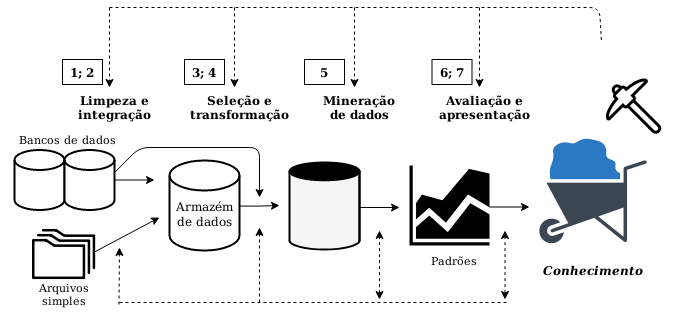
\includegraphics[width=0.85\textwidth]{img/based-on-figure-1-4-han-2011.png}
    \end{center}
    \vspace{-0.5cm}
    \legend{\ABNTEXfontereduzida \textbf{Fonte:} Figura baseada na original de \citeonline[p.~7]{Han:2011:DMC:1972541}.}
    \label{fig:diagrama-mineração-texto-han}
\end{figure}
    
    É importante notar essas 7 etapas de desenvolvimento de Mineração de Dados para abordamos a definição de MT, pois essa deriva muitas técnicas desenvolvidas na pesquisa do campo de Mineração de Dados para seu campo de aplicação, logo sistemas baseados em ambas áreas vão apresentar similaridades estruturais \cite[p.~1]{Feldman:2006:TMH:1076381}. 
    
    % Text mining can be broadly defined as a knowledge-intensive process in which a user interacts with a document collection over time by using a suite of analysis tools. In a manner analogous to data mining, text mining seeks to extract useful information from data sources through the identification and exploration of interesting patterns.
    
    % Because data mining assumes that data have already been stored in a structured format, much of its preprocessing focus falls on two critical tasks: Scrubbing and normalizing data and creating extensive numbers of table joins. In contrast, for text mining systems, preprocessing operations center on the identification and extraction of representative features for natural language documents. These preprocessing operations are responsible for transforming unstructured data stored in document collections into a more explicitly structured intermediate format, which is a concern that is not relevant for most data mining systems.
    
    A Mineração de Dados assume que os dados, que vão ser tratados durante seu processo, já foram armazenados em um formato estruturado, logo a maior parte de seu pré-processamento vai estar ligado às etapas 1 e 2 do processo de KDD citado, as de limpeza e integração dos dados \cite[p.~1]{Feldman:2006:TMH:1076381}. % Talvez seja necessário ao falar de linguagem natural dar um exemplo e um contra exemplo? Português e Java?
    Já na MT, como os dados de trabalho são textos, sendo texto configurado como dados desestruturados que consistem de \textit{strings} (palavras) organizadas de forma coerente e sendo pertencentes a uma linguagem natural \cite[p.~1]{Jo2018TMCIBDC}, temos que as operações de pré-processamento vão estar mais focadas em etapas adicionais, prévias às citadas para o processo de KDD, sendo estas novas direcionadas à identificação e extração de \textit{features} (atributos) representativas para documentos escritos em linguagem natural, transformando os dados não estruturados, que estão armazenados em coleções de documentos, em um formato mais explicitamente estruturado \cite[p.~1]{Feldman:2006:TMH:1076381}.
    % Text is defined as the unstructured data which consists of strings which are called words [82]
    
    
    % Na década de 70 houve o surgimento de diversas técnicas de gerenciamento de banco de dados, como por exemplo a 
    
    % -- Utiliza de várias áreas, falar delas
    % -- Utiliza das técnicas de RI para indexar os textos em algumas de suas aplicações
    % Text mining preprocessing operations include a variety of different types of techniques culled and adapted from information retrieval, information extraction, and computational linguistics research that transform raw, unstructured, original-format content (like that which can be downloaded from PubMed) into a carefully structured, intermediate data format. Knowledge discovery operations, in turn, are operated against this specially structured intermediate representation of the original document collection.
    
    As operações de pré-processamento para MT utilizam várias técnicas adaptadas dos campos de Recuperação de Informação, extração de informação e linguística computacional para transformar as coleções de documentos desestruturados em dados intermediários cuidadosamente estruturados \cite[p.~2--3]{Feldman:2006:TMH:1076381}. 
    Essa estrutura intermediária é definida por um modelo representacional dos documentos de texto composto por um conjunto de atributos, sendo sempre preferidos os modelos com menor número de variáveis significativas para a representação \cite[p.~4]{Feldman:2006:TMH:1076381}.
    % In Table 1.1, the differences between the mining and the retrieval are presented. The output of data mining is the implicit knowledge which is necessary directly for making decisions, whereas that of retrieval is some of data items which are relevant to the given query. For example, in the domain of stock prices, the prediction of future stock prices is a typical task of data mining, whereas taking some of past and current stock prices is that of information retrieval. Note that the perfect certainty never exists in the data mining, compared to the retrieval. The more advanced computation for making knowledge from the raw data, which is called synthesis, is required for doing the data mining tasks.
    
    Apesar da Mineração de Texto utilizar de técnicas da Recuperação de Informação, ambos são campos independentes com objetivos diferentes conforme ressalta \citeonline[p.~4, tradução nossa]{Jo2018TMCIBDC} (apresentados de modo resumido na Tabela \ref{tab:mineração-vs-recuperação}):

    \begin{citacao}
        A saída da mineração de dados é o conhecimento implícito que é necessário diretamente para a tomada de decisões, enquanto a saída da recuperação é composta por alguns dos itens de dados que são relevantes para a consulta dada. 
        Por exemplo, no domínio de preços de ações, a previsão dos preços futuros de ações é uma tarefa típica da mineração de dados, enquanto que obter alguns dos preços de ações passadas e atuais é tarefa da recuperação de informação. 
        Observe que a certeza perfeita nunca existe na mineração de dados, em comparação com a recuperação. 
        A computação mais avançada para obter conhecimento dos dados brutos, chamada de síntese, é necessária para executar as tarefas de mineração de dados.
    \end{citacao}
    
    \begin{table}[H]
    \centering
    \caption{Mineração de Dados versus Recuperação de Informação (em específico para objetos de texto a comparação vale para Mineração de Texto versus Recuperação de Texto).}
    \begin{tabular}{|l|l|l|}
        \hline
         
        & \makecell[l]{\textbf{Mineração}}
        & \makecell[l]{\textbf{Recuperação}}
        \\ \hline
        Saída
        & Conhecimento 
        & Itens relevantes
        \\ \hline
        Exemplo
        & Valores previstos 
        & Valores anteriores ou atuais
        \\ \hline
        Certeza
        & Probabilística 
        & Nítida
        \\ \hline
        Síntese
        & Necessária 
        & Opcional
        \\ 
        \hline
    \end{tabular}
    \legend{\ABNTEXfontereduzida \textbf{Fonte:} \citeonline[p.~4]{Jo2018TMCIBDC}}
    \label{tab:mineração-vs-recuperação}
\end{table}
    % Ressaltar denovo o suporte que a RI dá à MT, e então apresentar a diferenciação que Jo2018 faz na tabela 1.1 pag 4, e talvez a perspectiva do usuário apresentada por Zhai2016 a qual diferencia a Recuperação de Informação como Acesso dando poder de Selecionar Informação, e Mineração de Texto como Mineração possibilitando Criar Conhecimento, ele ainda apresenta a parte da Clusterização como Organização possibilitando Adicionar Estruturas/Marcações
    % Pensei em aqui contextualizar um pouco sobre os diversos campos que dão suporte ao KDD (Mineração de Dados) e à MT e colocar uma imagem parecida com a do \cite{Han:2011:DMC:1972541} na página 23 para mostrar os campos que dão suporte a MT
    
    A definição dos atributos para MT busca tirar proveito dos mais variados elementos presentes em um documento escrito em linguagem natural, no entanto é necessário um cuidado pois existe um grande número de palavras, frases e outros artefatos que podem comprometer o desempenho de um sistema de Mineração de Texto ou tornar a tarefa infactível \cite[p.~4]{Feldman:2006:TMH:1076381}, por isso a necessidade de identificar os melhores atributos, que trazem mais informação sobre o texto. 
    Nesse ponto que a MT pode se auxiliar de técnicas de RI para incrementar seu grupo de atributos, sendo alguns, como por exemplo o BM25 para RI ranqueada, utilizadas em competições de identificação de perfil de autores \cite{WEREN_MESTRADO_2014,WEREN_CLEF_2014,WEREN_ARTIGO_2014}. % procurar outros!!!!!.
    
    % -- Já devo diferenciar aqui
    
    % Falta falar de:
    % * Feature Engineering
    %  ---> Falar da definição mais ampla, feature selection, extraction, etc.
    % * Medidas de avaliação
    
    \subsection{Corpus} \label{subsec:Corpus}
    % Jo2018 - página 6 TEXT FORMATS
        Vários formatos de texto são utilizados para o processamento computacional de texto, segundo \citeonline[p.~6]{Jo2018TMCIBDC} os mais populares são os distribuídos pelo \textit{software} de escritório proprietário MS Office, como o arquivo padrão do MS Word com extensão ``doc'', MS PowerPoint com extensão ``ppt'', e o MS Excel com o ``xls'', e ainda para transferência entre computadores o mais utilizado é o formato PDF (\textit{Portable Document Format}).
        Como alternativa aos formatos proprietários do MS Office, foi aprovada a norma ISO/IEC 263000 em 8 de maio de 2006 que define o formato aberto ODF (\textit{Open Document Format for Office Applications}).
        A partir da padronização feita com o ODF são definidas diversas extensões que passaram a ser suportadas por praticamente todos os \textit{softwares} de escritório, como por exemplo a extensão ``.odt'' para documentos de texto, ``.ods'' para folhas de cálculo e ``.odp'' para apresentações.
        
        \begin{figure}[ht]
    \centering
    \caption{Arquivo de texto simples, texto não formatado, aberto para edição no xed.}
    \begin{center}
        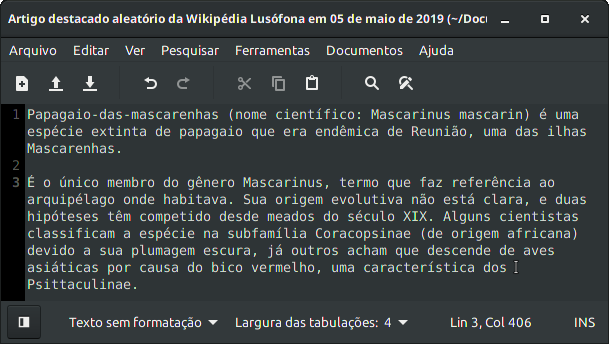
\includegraphics[width=0.75\textwidth]{img/exemplo-texto-simples.png}
    \end{center}
    \vspace{-0.5cm}
    \legend{\ABNTEXfontereduzida \textbf{Fonte:} O autor, conteúdo do texto obtido de \citeonline{Wikipedia_ConteudoDest05maio_2019}.}
    \label{fig:exemplo-texto-simples}
\end{figure}


        
        O texto simples, ou texto sem formatação, é o formato mais elementar de texto que é feito por um editor de texto, exemplificado na Figura \ref{fig:exemplo-texto-simples} por um arquivo aberto no editor xed\footnote{xed é um editor de texto leve e pequeno feito para o X-Apps \cite{LinuxMintXed2019}.}.
        Usualmente cada texto corresponde a único arquivo, sendo geralmente armazenado com a extensão ``txt'' nos sistemas operacionais Windows \cite[p.~6]{Jo2018TMCIBDC}.
        
        O XML (\textit{Extensive Markup Language}) pode ser considerado como outro formato de texto conforme exibido na Figura \ref{fig:exemplo-arquivo-xml}. 
        É o formato de documento \textit{web} mais flexível e foi projetado com base no HTML, o XML 1.0 foi padronizado pela W3C (\textit{World Wide Web Consortium}) em sua primeira versão em 1998, sendo a quinta edição a mais recente publicada em novembro de 2008 \cite{XML10_5ed_2008}.
        Atualmente o XML é utilizado como padrão para descrever itens de dados textuais de forma relacional, onde cada campo possui uma etiqueta de início e de fim, e o valor do campo fica entre estas etiquetas \cite[p.~6]{Jo2018TMCIBDC}.
        
        \begin{figure}[ht]
    \centering
    \caption{Exemplo de documento XML aberto no editor xed.}
    \begin{center}
        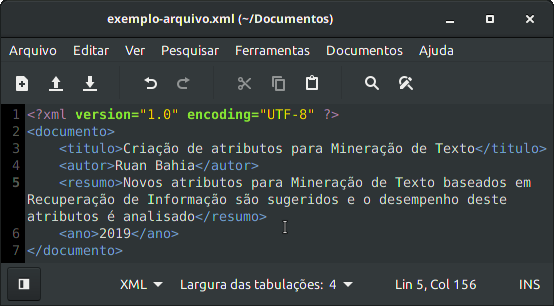
\includegraphics[width=0.65\textwidth]{img/exemplo-arquivo-xml.png}
    \end{center}
    \vspace{-0.5cm}
    \legend{\ABNTEXfontereduzida \textbf{Fonte:} O autor.}
    \label{fig:exemplo-arquivo-xml}
\end{figure}
        
        Uma coleção de textos simples é chamada de corpus, geralmente sendo referenciado pelo diretório que contém os arquivos de texto, e excepcionalmente um único arquivo pode também corresponder a um corpus ao invés de ser somente um único arquivo de texto \cite[p.~6]{Jo2018TMCIBDC}.
        Num conceito mais abrangente, \citeonline[p.~9]{KwartlerTMPWR2017} considera como corpus qualquer corpo, ou conjunto, grande de texto organizado, assim um conjunto de arquivos de texto XML também é tratado como um corpus.
    
    \subsection{Tarefas de Mineração de Dados} \label{subsec:Tarefas-de-Mineração-de-Dados}
        As tarefas de Mineração de Dados podem ser divididas em duas categorias, segundo \citeonline[p.~7]{TanIDM2014} e \citeonline[p.~15]{Han:2011:DMC:1972541}: 
        \begin{itemize}
            \item \textbf{Descritivas}: tem como objetivo caracterizar propriedades dos dados no conjunto objetivo por meio da derivação de padrões que resumem as relações nos dados; e
            
            \item \textbf{Preditivas}: realizam uma indução nos dados presentes objetivando prever valores de um atributo em particular, sendo este atributo a ser previsto chamado de objetivo. 
        \end{itemize}
        
        Quanto às tarefas em si, a mineração de dados possui tarefas de agrupamento, associação, classificação, descrição, detecção de anomalias, e de regressão.
        As quatro principais estão ilustradas na Figura \ref{fig:tarefas-principais-mineração-dados}.
        As tarefas de classificação e de regressão entram na categoria de tarefas preditivas, e são às vezes referidas como tarefas de modelagem preditiva. 
        Ainda, tarefas de classificação trabalham com atributos objetivos discretos, enquanto que tarefas de regressão tem seus atributos objetivos como variáveis contínuas \cite[p.~7--8]{TanIDM2014}, e ambas focam na análise de conjuntos de dados rotulados, os chamados de conjuntos de treinamento \cite[p.~19]{Han:2011:DMC:1972541}.
        Na Mineração de Textos uma tarefa de classificação normalmente recebe o nome de \textbf{categorização de texto} \cite[p.~6]{TurchiATPUKM2009} \cite[p.~61]{Feldman:2006:TMH:1076381}.
        
        \begin{figure}[ht]
    \centering
    \caption{As quatro principais tarefas da mineração de dados.}
    \begin{center}
        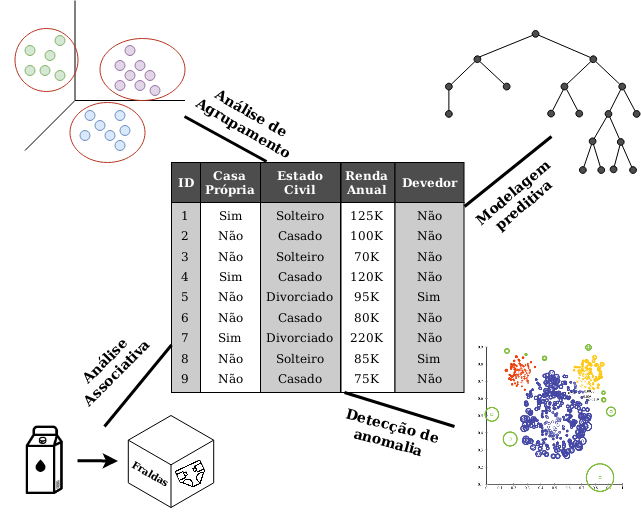
\includegraphics[width=0.85\textwidth]{img/tarefas-principais-mineracao-dados.png}
    \end{center}
    \vspace{-0.5cm}
    \legend{\ABNTEXfontereduzida \textbf{Fonte:} Figura baseada na original de \citeonline[p.~7]{TanIDM2014}.}
    \label{fig:tarefas-principais-mineração-dados}
\end{figure}


        
        Segundo os autores \citeonline[p.~15--21]{Han:2011:DMC:1972541}, \citeonline[p.~8--11]{TanIDM2014} e \citeonline[p.~8--14]{LaroseDKD2014} as demais tarefas da mineração de dados são descritivas e podem ser caracterizadas como segue:
        \begin{itemize}
            \item \textbf{Agrupamento}: consiste numa análise dos dados sem consulta à rótulos de classe, podendo estes até não estarem presentes, e este tipo de tarefa é utilizada para gerar rótulos de classes para grupos de dados. 
            Na literatura é mais comum se referir ao termo em língua inglesa, \textit{clustering};
            
            \item \textbf{Associação}: são descobertos relacionamentos mais frequentes entre os atributos, utilizada para descoberta de padrões, geralmente por meio de regras de implicação;
            
            \item \textbf{Descrição}: os dados são associados com conceitos, consistindo da caracterização dos dados, no qual é feito o resumo das características gerais de uma classe objetivo; 
            ou da discriminação dos dados, na qual é feita a comparação, contraste, dos atributos de uma classe objetivo com um conjunto de outras classes;
            
            \item \textbf{Detecção de anomalias}: também chamado de detecção de dados discrepantes (\textit{outliers}), foca na identificação de exemplos dos dados que possuem características significativamente diferentes do restante. 
            Muitos métodos de mineração de dados descartam os \textit{outliers} por considerarem estes como ruídos nos dados.
        \end{itemize}
    
        \subsubsection{Classificação binária} \label{subsubsec:Classificação-binária}
            O problema da classificação consiste na aprendizagem da estrutura dos exemplos do conjunto de dados, os quais estão classificados em grupos chamados de categorias ou classes \cite[p.~285]{Aggarwal_DMTT_2015}.
            A entrada consiste de uma coleção de registros, conhecidos como exemplos, cada um caracterizado pela tupla $(\textbf{x},y)$ onde $\textbf{x}$ é um conjunto de atributos e \textit{y} é o atributo chamado de rótulo da classe.
            \citeonline[p.~146, tradução nossa]{TanIDM2014} dizem que ``classificação é a tarefa de aprender uma função objetivo $f$ que mapeia cada conjunto de atributos $x$ a um rótulo de classe predefinido $y$''.
        % Definition 4.1 (Classification). Classification is the task of learning a target function f that maps each attribute set x to one of the predefined class labels y.
        % The target function is also known informally as a classification model. A classification model is useful for the following purposes.
        
            O aprendizado da função objetivo é feito com um modelo, chamado de modelo de treinamento, pois este é baseado no conjunto de treinamento. 
            Então, este modelo de treinamento é utilizado para prever a classe de exemplos não vistos anteriormente, isso quer dizer que estes exemplos não fazem parte do conjunto de treinamento.
            Segundo \citeonline[p.~286, tradução nossa]{Aggarwal_DMTT_2015}, então, a maior parte dos algoritmos de classificação possui duas fases:
            \begin{enumerate}
                \item \textbf{Fase de treinamento}: nessa fase um modelo de treinamento é construído à parte das instâncias de treinamento. Isto pode ser entendido, intuitivamente, como um resumo do modelo matemático dos grupos rotulados no conjunto de dados de treinamento;
                
                \item \textbf{Fase de teste}: nessa fase o modelo de treinamento é utilizado para determinar os rótulos de classe (ou identificadores de grupos) de uma ou mais instâncias não vistas.
            \end{enumerate}
                
            A tarefa de classificação é também chamada de aprendizado supervisionado porque exemplos dos dados são utilizados para aprender as estruturas de agrupamento das classes \cite[p.~285]{Aggarwal_DMTT_2015}.
            Técnicas de classificação são mais apropriadas para dados com categorias binárias ou nominais, não sendo indicados para categorias com significado ordinal, pois a tarefa de classificação não considera a ordem implícita entre as categorias \cite[p.~147]{TanIDM2014}.
            A tarefa de categorização dos dados pode ser com rótulo único ou com múltiplos rótulos, na categorização com múltiplos rótulos as categorias se sobrepõem, e já na categorização com rótulo único cada exemplo de dado pertence a exatamente uma categoria \cite[p.~67]{Feldman:2006:TMH:1076381} \cite[p.~306]{TanIDM2014}.
            
            A classificação binária é um caso especial da categorização de rótulo único na qual quantidade de categorias é dois, sendo este o caso mais simples das tarefas de classificação, pois nele só existem duas possibilidades de rótulo de classe e cada objeto de dados pertence, exclusivamente, a uma das classes \cite[p.~67]{Feldman:2006:TMH:1076381} \cite[p.~81]{Jo2018TMCIBDC}.
            Um exemplo clássico de categorização binária de texto é um analisador de \textit{spam}\footnote{Conteúdo indesejado, tratado como lixo eletrônico.} para e-mails, nele só existem duas possibilidades de classificação para dado e-mail, ou \textbf{é \textit{spam}} ou \textbf{não é \textit{spam}}.
        
    \subsection{Engenharia de atributos} \label{subsec:Engenharia-de-atributos}
        % Falar do sentido amplo da feature engineering, abrangindo feature extraction, creation, selection, etc.
        O processo para extrair atributos passíveis de serem utilizados por classificadores da mineração de dados é chamado por \citeonline{ZhengFEML2018} de \textit{feature engineering}, que em uma tradução livre tentando preservar o contexto pode ser chamado de \textit{manejo de atributos}.
        Num conceito mais generalista, \citeonline[p.~3, tradução nossa]{DongFEMLDA2018} define \textit{feature engineering} como uma área que abrange ``os tópicos de transformação de atributos, geração de atributos, extração de atributos, seleção de atributos, análise e avaliação de atributos, metodologias de manejo generalista e automatizado de atributos, e aplicações do manejo de atributos'', sendo essa a definição de engenharia de atributos no processo de KDD.
        
        Cada um dos tópicos da engenharia de atributos é definido por \citeonline[p.~3]{DongFEMLDA2018} como segue:
        \begin{itemize}
            \item \textbf{Transformação de atributos}: construção de novos atributos a partir de atributos existentes, frequentemente feito por meio de mapeamentos matemáticos;
            
            \item \textbf{Geração de atributos}: também chamado de criação de atributos ou de extração de atributos, é  a geração de novos atributos que não são resultados de transformações. 
            Por exemplo, atributos derivados de padrões e de técnicas de domínio específico se encontram na categoria de geração de atributos;
            
            \item \textbf{Seleção de atributos}: selecionar um pequeno conjunto de atributos dentre um montante, com objetivo de reduzir o conjunto de atributos para tornar a tarefa de classificação computacionalmente viável. 
            A seleção de atributos também pode visar medição de atributos úteis e a melhora do desempenho por meio da escolha do melhor subconjunto;
            
            \item \textbf{Metodologias de manejo generalista e automatizado de atributos}: abordagens para geração automática de uma grande quantidade de atributos e seleção de um subconjunto dentre os atributos gerados;
            
            \item \textbf{Aplicações do manejo de atributos}: a utilização das técnicas de engenharia de atributos para resolver outras tarefas de análise de dados.
        \end{itemize}

        \subsubsection{Atributos comuns para documentos} \label{subsubsec:Atributos-comuns-documentos}
            % Feldman2006 apresenta esses atributos básicos nas páginas 4--7
            Ao atacar um problema de MT em uma coleção de documentos é de suma importância a definição dos atributos a serem utilizados na tarefa, e mesmo em pequenas coleções o problema da alta dimensionalidade dos atributos aparece.
            \citeonline[p.~4, tradução nossa]{Feldman:2006:TMH:1076381} exemplificam que até mesmo ``em uma coleção extremamente pequena de 15 mil documentos selecionados de notícias da Reuters, podem ser identificadas mais de 25 mil raízes de palavras não triviais''.
            
            A alta dimensionalidade dos atributos pode aparecer como um empecilho computacional para a realização da MT, por fazer com que os cálculos necessários sejam muito mais demorados e em alguns casos tornando-se um problema computacionalmente inviável.
            Então, a identificação e escolha de um modelo representacional, um bom conjunto de atributos, para representar os documento é algo de suma importância \cite[p.~4]{Feldman:2006:TMH:1076381}.
            
            Os tipos de atributos mais utilizados para representar documentos, segundo  \citeonline[p.~5--7]{Feldman:2006:TMH:1076381}:
            \begin{itemize}
                \item \textbf{Caracteres}: são as letras, números, e caracteres especiais presentes nos documentos utilizados para construir a semântica do mesmo;
                
                \item \textbf{Palavras}: são símbolos linguísticos nativos do espaço de atributos de um documento. 
                Atributos a nível de palavra geralmente são palavras únicas selecionadas de um documento nativo, e também é possível que sejam utilizados todas as palavras de um documento para representá-lo;
                
                \item \textbf{Termos}: são palavras únicas e frases com mais de uma palavra selecionadas de um corpus de documentos nativos por meio de técnicas específicas para extração de termos;
                
                \item \textbf{Conceitos}: são os atributos gerados de modo manual, baseado em regras, ou via categorização híbrida feita no pré-processamento. 
                Por exemplo, um documento sobre carros esportivos pode não incluir a palavra ``automóvel'', mas este conceito pode ser utilizado para identificar e representar esse documento.
            \end{itemize}
            
            
       \subsubsection{Criação de atributos} \label{subsubsec:Criação-de-atributos} 
            A criação de atributos também é referida como geração de atributos, e consiste em derivar novos conjuntos de atributos que capturem, de forma mais efetiva, a informação carregada pelos dados \cite[p.~55]{TanIDM2014}.
            
            Algumas metodologias de criação de atributos são apresentadas por \citeonline[p.~55--57]{TanIDM2014}:
            \begin{itemize}
                \item \textbf{Extração de atributos}: a criação de um novo conjunto de atributos a partir dos dados brutos.
                Por exemplo, no domínio da classificação de imagens os dados brutos são os \textit{pixels}, que não são apropriados para tarefas de classificação, no entanto os dados podem ser processados para fornecer informações de presença de contornos, que podem então ser utilizados por técnicas de classificação para identificar rostos;
                
                \item \textbf{Mapeamento dos dados para um novo espaço}: mudar completamente a visualização dos dados.
                Considerando uma série temporal, por exemplo, os dados podem ser transformados na informação de frequência dessa série por meio da transformada de Fourier;
                
                \item \textbf{Construção de atributos}: os atributos presentes nos dados possuem a informação necessária para o processo de mineração, mas não estão na forma adequada, assim novos atributos podem ser construídos na forma adequada.
                Um exemplo é a construção de um atributo de densidade em uma tarefa de classificação na qual os dados contém informação de volume e massa de itens.
            \end{itemize}
            
        
    \subsection{Medidas de avaliação de classificadores} \label{subsec:Medidas-de-avaliação-de-classificadores}
    % Jo2018 - página 157 são algumas, pegar de Han2011 a parte de avaliação de modelo página 364
        Tarefas de classificação (categorização) de texto produzem modelos de classificadores, os quais tem efetividade avaliada em termos de suas medidas de \textbf{precisão} e de \textbf{revocação}\footnote{As medidas na língua inglesa são chamadas de \textit{precision} e \textit{recall}.} \cite[p.~48]{Berry2010TMAT}, e também há uma preocupação grande com a \textbf{acurácia} do classificador \cite[p.~313]{Zhai2016TDMA}.
        As medidas de avaliação de um modelo de classificador devem ser calculadas com base na aplicação do modelo num conjunto de teste, consistindo de tuplas não utilizadas para treinar o modelo \cite[p.~364]{Han:2011:DMC:1972541}.
        
        Antes de descrever as medidas, é necessário abordar o conceito de exemplos positivos (ou tuplas positivas) e de exemplos negativos (ou tuplas negativas) nos dados a serem classificados. 
        Os exemplos positivos são aqueles da classe de maior interesse, e os exemplos negativos são todos o restante \cite[p.~364]{Han:2011:DMC:1972541}.
        Considerando uma classificação binária, pode-se ter os exemplos positivos referentes a \textit{spam = sim} e os negativos \textit{spam = não}.
        Seguindo, como descrito por \cite[p.~364--365]{Han:2011:DMC:1972541}, ao construir um modelo de classificador treinado com exemplos deste tipo, e então ao testá-lo em um conjunto com a classe objetivo conhecida, serão previstas as classes desse conjunto.
        Sendo $P'$ o número de exemplos classificados positivamente, e $N'$ o número de exemplos classificados negativamente. 
        Cada exemplo pode então ter a classe prevista comparada com as classes objetivos já conhecidas, gerando a matriz de confusão da Tabela \ref{tab:matriz-confusão} como um sumário das previsões corretas e incorretas.
                % falar que a matriz de confusão pode ter mais linhas e colunas


        \begin{table}[H]
    \centering
    \caption{Matriz de confusão para uma tarefa de classificação binária, exibida com os totais para exemplos positivos e negativos.}
    \begin{adjustbox}{max width={\textwidth},keepaspectratio}%
    \begin{tabular}{p{1.2cm}|p{1.2cm}|p{1.2cm}|p{1.2cm}|p{1.2cm}}
        \multicolumn{2}{c}{} 
        & \multicolumn{2}{c}{\textbf{Classe prevista}} 
        \\ \cline{3-4}
        \multicolumn{2}{c|}{}
        & \makecell[c]{\textit{sim}}
        & \makecell[c]{\textit{não}}
        & \makecell[c]{Total}
        \\ \cline{2-4}
        \multirow{2}{1.2cm}{
            \rotatebox{90}{
                \parbox{1.4cm}{\centering \textbf{Classe real}}
            }
        }
        & \makecell[c]{\textit{sim}} 
        & \makecell[c]{\textit{TP}} 
        & \makecell[c]{\textit{FN}} 
        & \makecell[c]{$P$}
        \\ \cline{2-4}
        
        & \makecell[c]{\textit{não}} 
        & \makecell[c]{\textit{FP}}
        & \makecell[c]{\textit{TN}}
        & \makecell[c]{$N$}
        \\ \cline{2-4}
        \multicolumn{1}{c}{}
        & \multicolumn{1}{c}{Total} 
        & \multicolumn{1}{c}{$P`$}
        & \multicolumn{1}{c}{$N`$}
        & \multicolumn{1}{c}{$P + N$}
        \\
    \end{tabular}
    \end{adjustbox}
    \legend{\ABNTEXfontereduzida \textbf{Fonte:} Tabela disponível em \citeonline[p.~366]{Han:2011:DMC:1972541}.}
    \label{tab:matriz-confusão}
\end{table}
        
        A matriz de confusão tem tamanho $n \times n$, onde $n$ é o número de classes (sempre maior ou igual a 2).
        Cada entrada ${MC}_{i,j}$ da matriz corresponde ao número de exemplos da classe $i$ rotulado pelo classificador como pertecente à classe $j$.
        A terminologia utiliza na Tabela \ref{tab:matriz-confusão}, caso específico para classificação binária, possui o seguinte significado:
        \begin{itemize}
            \item \textbf{Verdadeiros positivos} (\textit{TP}): referente ao número de exemplos positivos rotulados corretamente;
            
            \item \textbf{Verdadeiros negativos} (\textit{TN}): número de exemplos negativos rotulados corretamente;
            
            \item \textbf{Falsos positivos} (\textit{FP}): número de exemplos positivos rotulados incorretamente, a classe real na verdade era negativa, no entanto o modelo de classificação rotulou como a classe positiva;
            
            \item \textbf{Falsos negativos} (\textit{FN}): número de exemplos negativos rotulados incorretamente, por exemplo a rotulação de um exemplo como \textit{spam = não} sendo que sua classe real na verdade é \textit{spam = sim}.
        \end{itemize}
        A adição de totais à matriz de confusão é comum \cite[p.~366]{Han:2011:DMC:1972541}, na matriz apresentada na Tabela \ref{tab:matriz-confusão} estão apresentados os totais $P'$ e $N'$, respectivamente o número total de exemplos rotulados como positivos ($\textit{TP} + \textit{FP}$) e o número de exemplos rotulados como negativos ($\textit{TN} + \textit{FN}$).
        $P$ é o número de exemplos com classe real positiva ($\textit{TP} + \textit{FN}$) e $N$ é o número de exemplos com classe real negativa ($\textit{FP} + \textit{TN}$).
        
        A razão entre o número de classificações verdadeiras positivas e o número classificações positivas dá a precisão ($p$) do classificador, conforme mostra a Equação \ref{eq:medida-precisão}, e segundo \citeonline[p.~368, tradução nossa]{Han:2011:DMC:1972541} ``precisão pode ser pensada como uma medida de exatidão''.
        
        A revocação ($r$) é dada pela Equação \ref{eq:medida-revocação}, que é a razão entre o número o número de classificações verdadeiras positivas e o número de exemplos positivos da classe real, e também é chamada de sensitividade \cite[p.~364--365]{Han:2011:DMC:1972541}.
        Ainda, segundo  \citeonline[p.~368, tradução nossa]{Han:2011:DMC:1972541} ``revocação é uma medida de completude''.
        
        \vspace{\parskip}
        \noindent\begin{minipage}{.5\textwidth}
            \begin{equation}
                \label{eq:medida-precisão}
        		p = 
        		\frac{\textit{TP}}{\textit{TP} + \textit{FP}}
        		= \frac{\textit{TP}}{P'}
            \end{equation}
        \end{minipage}
        \begin{minipage}{.5\textwidth}
            \begin{equation}
                \label{eq:medida-revocação}
        		r = 
        		\frac{\textit{TP}}{\textit{TP} + \textit{FN}}
        		= \frac{\textit{TP}}{P}
            \end{equation}
        \end{minipage}
        \vspace{\parskip}
        
        As medidas de precisão e revocação podem ser combinadas em uma única medida chamada de $F$ (também conhecida como $F$-\textit{score} ou pontuação ${F_1}$), que é a média harmônica entre elas, definida como disposto na Equação \ref{eq:medida-f-score}.

        O nível geral de reconhecimento do classificador é medido pela acurácia ($acc$), que é definida pela Equação \ref{eq:medida-acurácia}, representando a razão de exemplos do conjunto de teste que foram classificados corretamente.
        
        \vspace{\parskip}
        \noindent\begin{minipage}{.5\textwidth}
            \begin{equation}
                \label{eq:medida-f-score}
        		F = 
        		\frac{2 \times p \times r}{p + r}
            \end{equation}
        \end{minipage}
        \begin{minipage}{.5\textwidth}
            \begin{equation}
                \label{eq:medida-acurácia}
        		acc = 
        		\frac{\textit{TP} + \textit{TN}}{P + N}
            \end{equation}
        \end{minipage}
        \vspace{\parskip}
        
        Apesar das medidas $F$, precisão, revocação e acurácia serem bastante úteis na medida de efetividade de classificadores, \citeonline[p.~48]{Berry2010TMAT} afirmam que elas não consideram o custo da classificação errônea em problemas com classes desbalanceadas, e então sugere um critério de acurácia ponderada e similarmente \citeonline[p.~369]{Han:2011:DMC:1972541} sugerem o uso da medida $F_\beta{}$ definida como descrito na Equação \ref{eq:medida-f-beta}.        \begin{equation}
            \label{eq:medida-f-beta}
    		F_\beta{} = 
    		\frac{(1 + \beta{}^2) \times p \times r}{\beta{}^2 \times p + r}
        \end{equation}
        
        As medidas de avaliação de classificadores possibilitam a comparação de diferentes modelos de classificadores e assim é possível efetuar a seleção do modelo, que é a escolha do melhor classificador dentre os modelos gerados para um problema específico \cite[p.~364]{Han:2011:DMC:1972541}.